%!TEX root = ../main.tex

% NOTES:
%   * There is a shift to accelerator design
%   * CPUs are inefficient
%   * Fixed accelerators are hard to program
%   * Alternative is FPGA/CGRA
%   * There are challenges with programming FPGA/CGRA
%   * HLS is one solution

%


\section{Abstraction Levels}

The growing capabilities of silicon technology over the previous decades has forced design methodologies and tools to move to higher levels of abstraction.
In order to explain the relationship between different design methodologies on different abstraction levels, we will use the Y-Chart~\cite{walker_1985_y_model}~\ref{fig:y-chart}.

\begin{figure}[h]
    \centering
    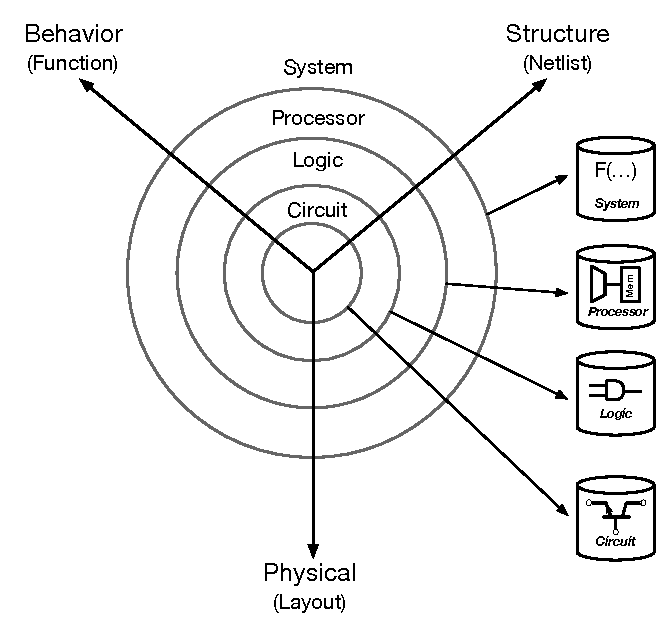
\includegraphics[width=0.5\textwidth]{figures/Introduction/Y-Chart.pdf}
    \caption{Y-Chart}
    \label{fig:y-chart}
\end{figure}

Y-Chart divides design representation into three domains, three axises on the chart:
1)The behavioral domain describes the behavior, or functionality, of the design, ideally without any reference to the way this behavior is achieved by an implementation.
Behavioral represents a design as a black-box but it describes the output base on inputs over time.
What behavior representation doesn't specify is how the black-box is structured or how to build the black-box.
2)The structural domain describes the abstract implementation, or logical structure, of the design as a hierarchy of components and their interconnections.
In this specification, black-box is represented as a set of components and connections.
While, it's possible to drive the behavior of black-box from its components and its connections but understanding the behavior can be very difficult since it is obscured by the details of each component and connection.
3)Physical, usually called layout or board design.
Physical design describe different dimension of each component.

The Y-chart contains three axises to represent design domains.
It also contains concentric circles to defines multiple level of abstractions for a design.
Gajski~\cite{gajski_1992_high} proposed four levels of abstraction: system, processor, logic and circuit levels.
In this model, the name of each abstraction level is derived from the types of the components generated on that abstraction level.
For instance, on the processor level, we generate general purpose and \emph{custom} processors, or \emph{special-hardware components} such as memory controllers, arbiters, bridges and various interface components.
At the higher level, system level, we design standard or embedded systems consisting of processors, memories, buses, and other processor components.
In the next two other level, we describe the circuit in terms of registers and the data transfer between the registers, logic level. Finally, circuit level or transistor level, implements the behavior of logic gates.
In the rest of this report we focus on only the first two level of abstraction, processor and system.

On each abstraction level, we need a library of components to be used in building \emph{the structure} for a given \emph{behavior}.
The process of converting the given behavior into a structure for a given haviour is called \textbf{synthesis}.
Once a structure is defined and verified, we can proceed to the next lower abstraction level by further synthesizing each components to their corresponding structure.
Thus, each component in the library may have up to three different models representing three different axes in the Y-Chart: behavior or function; structure, which contains the components from the lower level of abstraction and the physical.
Fortunately, to design a new hardware all three models for each component are not typically needed most of the time.
Most of the methodologies presently in use, which we are going to discuss in the next chapter, perform design or synthesis on the system and processor levels.
At these two levels, every system component except memories is synthesized to the logic level, before the physical design is performed on the logic level.
Once the design is represented in terms of logic gates, depending on the target backend, we can perform layout placement, routing and used standard cells for each logic components, like wires and registers.
On the other hand, some components on the processor-and-system levels may be obtained as IPs and not synthesized, for example DSP blocks in FPGAs.
Therefore, their structure and physical design are known, on the level higher than logic level.
In that case, the physical design then may contain components of different sizes and from different levels of abstraction.
In the rest of this report we focus on the first two level of abstractions: \textit{Processor} and \textit{System}, how these abstraction can be expressed a programming languages and the process of \emph{synthesis} at these two levels.


\section{Behavioral Model}
\label{sec:processor_level_behavioral_model}

On each abstraction level we design components with different granularity with programming languages. At the processor level, the core building block of design is processing elements (PEs).
PEs are computational components that we define and design to do operations.
Each PE can be either a dedicated or a custom component that computes some specific functions.
It can be a general, like ALU at processors, or standard PE that can compute any function specified in some standard programming language.
The functionality or behavior of each PE can be specified in several different ways.
In the basic implementation of PEs, their functionality can be specified with mathematical expressions or formulas.
However, there is no limitation on what the functionally of a PE can be.
Therefore, we can expand the functionality of a PE and specify it with an algorithm in some \textit{programming language}.
For instance, we can define three PEs with three different mathematical expression: $y = |b|$, $x = |a|$ and $z = max (x, y)$.
Using only mathematical expressions and PEs, however, to define different type of computation is not sufficient.
To go beyond a mathematical expression and add the notion of control, one possible solution is to use Finite State Machines (FSMs).
A FSM is defined with a set of states and a set of transitions from state to state, which are taken when some input variables reach the required value.
Furthermore, each FSM generates some values for output variables in each state or during each transition. A FSM model can be made clock-accurate if each state is considered to take one clock cycle.
Figure~\ref{fig:fsm_model} shows an example of a FSM which connected our three PEs.
The example FSM has three states, S1, S2, and S3, and arcs representing state changes under different inputs.
Each state executes a computation represented by one or more arithmetic expressions or programming statements.
For example, in state S1, the FSM in Figure~\ref{fig:fsm_model} computes two functions, $x = |a|$ and $y = |b|$, and in state S3 it computes the function $z = max (x, y)$.
Hardware Definition Languages (HDLs) like Verilog and VHDL have support for both mathematical expression to become PEs and FSM model to support control structures at their behavioral level.
But there is a limitation in FSM model that makes it insufficient to express different type of computations.
FSM model is usually not clock-accurate since computation in each state may take more than one clock cycle.
Hence, for representing computation expressed by programming languages like C, FSM model is not adequate and we need a more comprehensive model.


\begin{figure}[h]
    \centering
    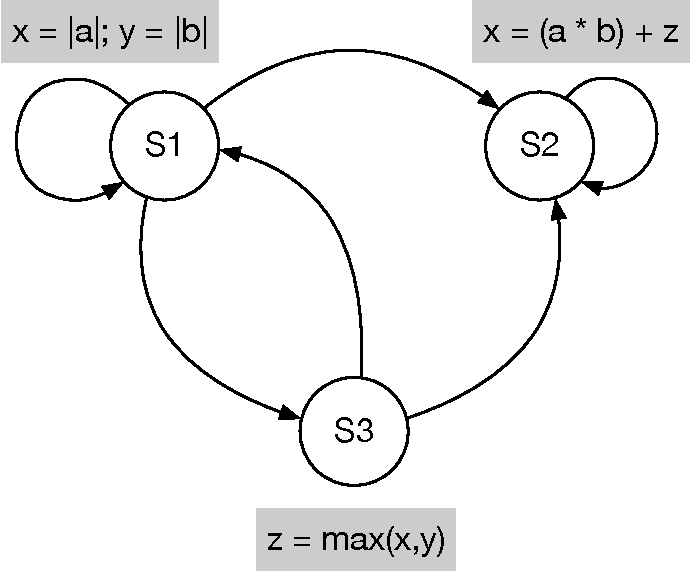
\includegraphics[width=0.4\textwidth]{figures/Introduction/FSM.pdf}
    \caption{FSM model}
    \label{fig:fsm_model}
\end{figure}


In general, programming languages consist of three elements: \code{if} statements, loops, and expressions.
An \code{if} statement has two parts, then and else, in which then is executed if the conditional expression given in the \code{if} statement is true, otherwise the \code{else} part is executed.
In each of the then or else parts, the \code{if} statement computes \emph{a set of expressions called a Basic Block (BB)}.
The \code{if} statement can also be used in the loop construct to represent loop iterations, which are executed as long as the condition in the \code{if} statement is true.
As a result, the combination of \code{if} statements, Control-Flow Graph (CFG) and BBs, Data-Flow Graph (DFG) can represent any programming-language code.
 
Figure~\ref{fig:c_example} shows an example of such a CFG and DFG combination. 
In this this example, we represent a loop with an \code{if} statement inside the loop iteration.
In each iteration, the loop construct executes BB1 and BB2 or BB3 depending on the value of \code{if} statement. At the end, the loop is exited if all all iterations are executed.

A Control-Data dependency graph shows explicitly the control dependencies between loop statements, if statements, and BBs, as well as the data dependences among operations inside a BB.
On can convert Control-Data dependency graph to a FSM by assigning a state to each BB and one state for the computation of each if conditional.
However, each state in such a FSM may need several clock cycles to execute its assigned BB or if condition.
Designing such FSM is challenging, we explain more in chapter 2.

\begin{listing}[!h]
    \begin{minipage}{0.5\textwidth}
        \begin{minted}{C++}
            for(int i = 0; i < N; i++){
                if(i % 2 == 0){
                    a = b + c;
                    b = c * 4;
                }
                else {
                    a = b - c;
                    c = b * 4;
                }
            }
        \end{minted}
    \end{minipage}
    \begin{minipage}{0.5\textwidth}
       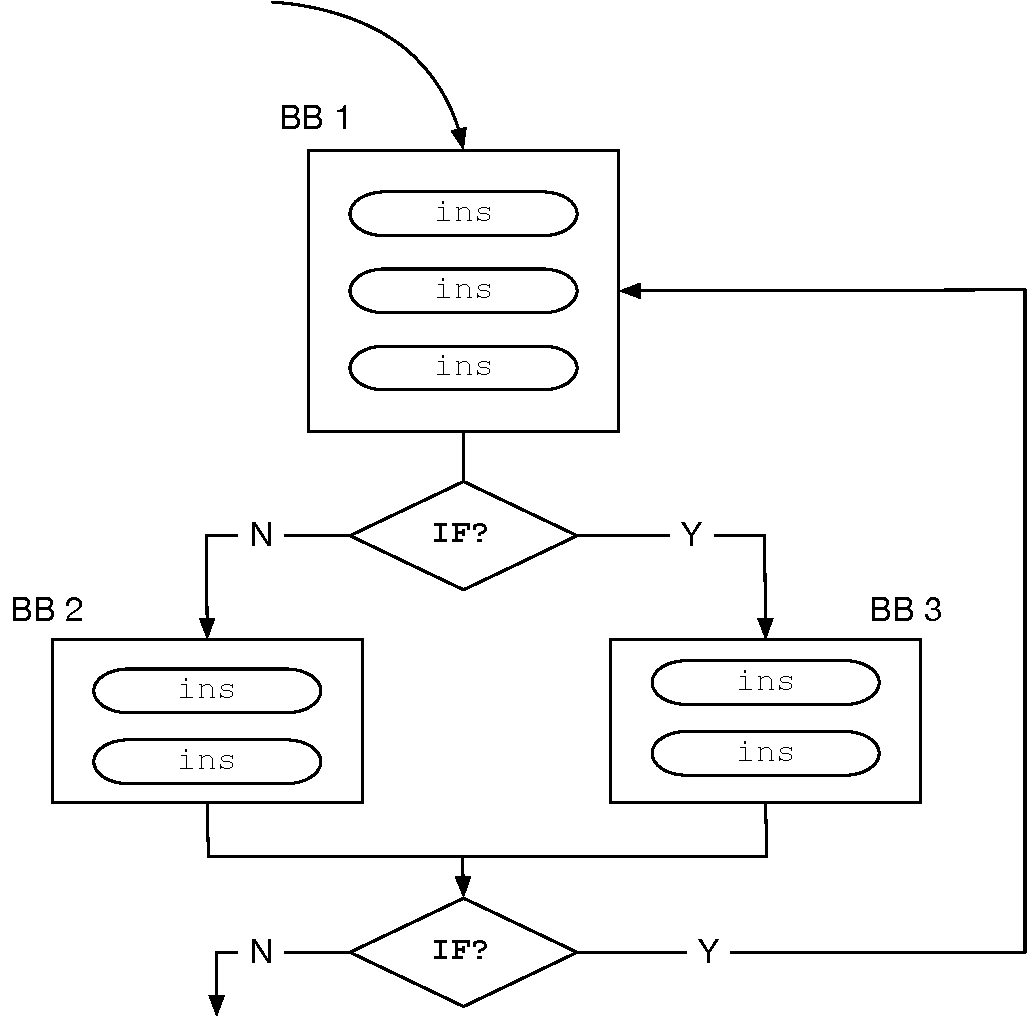
\includegraphics[width=0.85\textwidth]{figures/Introduction/CFG.pdf}
    \end{minipage}
    \caption{A C program example}
    \label{fig:c_example}
\end{listing}


While Control-Data dependency graph can be used to for specifying a single processor, but it is not suffice for describing a complete system that consist of many communicating processors.
A system-level model must represent multiple process running in parallel or in pipelined mode, with introducing notion of concurrency and pipelining.
Moreover, we need to have notion of synchronization since each processor can run concurrently and they may exchange data between each other.
Language extensions such as Cilk~\cite{cilk}/OpenMP and languages like Go with the notion of communication channels provide such mechanism to specify system level behavior at the software.

\section{Structural Model}

As we discussed a processor’s behavioral model, whether defined by a program in C, Control-Data dependency graph or FSM, \emph{can be implemented with a set of register-transfer components}.
In such a structural model usually there are a controller and a datapath like general purpose processors.
A datapath consists of three main component. 1) a set of storage elements such as register files, scratchpads, and memories, 2) a set of functional units such as ALUs, multipliers, shifters, and other custom functional units, and 3)a set of busses.
All of these components may be allocated in different quantities, size and types and connected arbitrarily through busses.
Each component may take one or more clock cycles to execute, each component may be pipelined, and each component may have input or output latches.
In addition, in many processor designs, the entire datapath is pipelined in several stages in addition to components being pipelined by themselves.
The choice of components and datapath structure depends on the metrics such as performance or energy to be optimized for a particular implementation.

The datapath does not work stand alone without a controller.
The controller defines the state of the processor and issues the control signals for the datapath at each cycle.
The structure of the controller and its implementation varies depending on whether the processor is a standard processor, like RISC processors, a custom-design processor like special image processing processors. 
Figure~\ref{fig:proc_structure} shows an example of such control and datapth for a simple 2 stage RISCV sodor core\footnote{\url{https://github.com/librecores/riscv-sodor/wiki}}.
In the case of a standard processor, the controller is programmable with a program counter (PC), and an address generator (AG) that defines the next address to be loaded into the PC.
In the case of specific custom processors, the controller can be implemented with programmability concepts typical of standard processors.



\begin{figure}[!t]
    \centering
    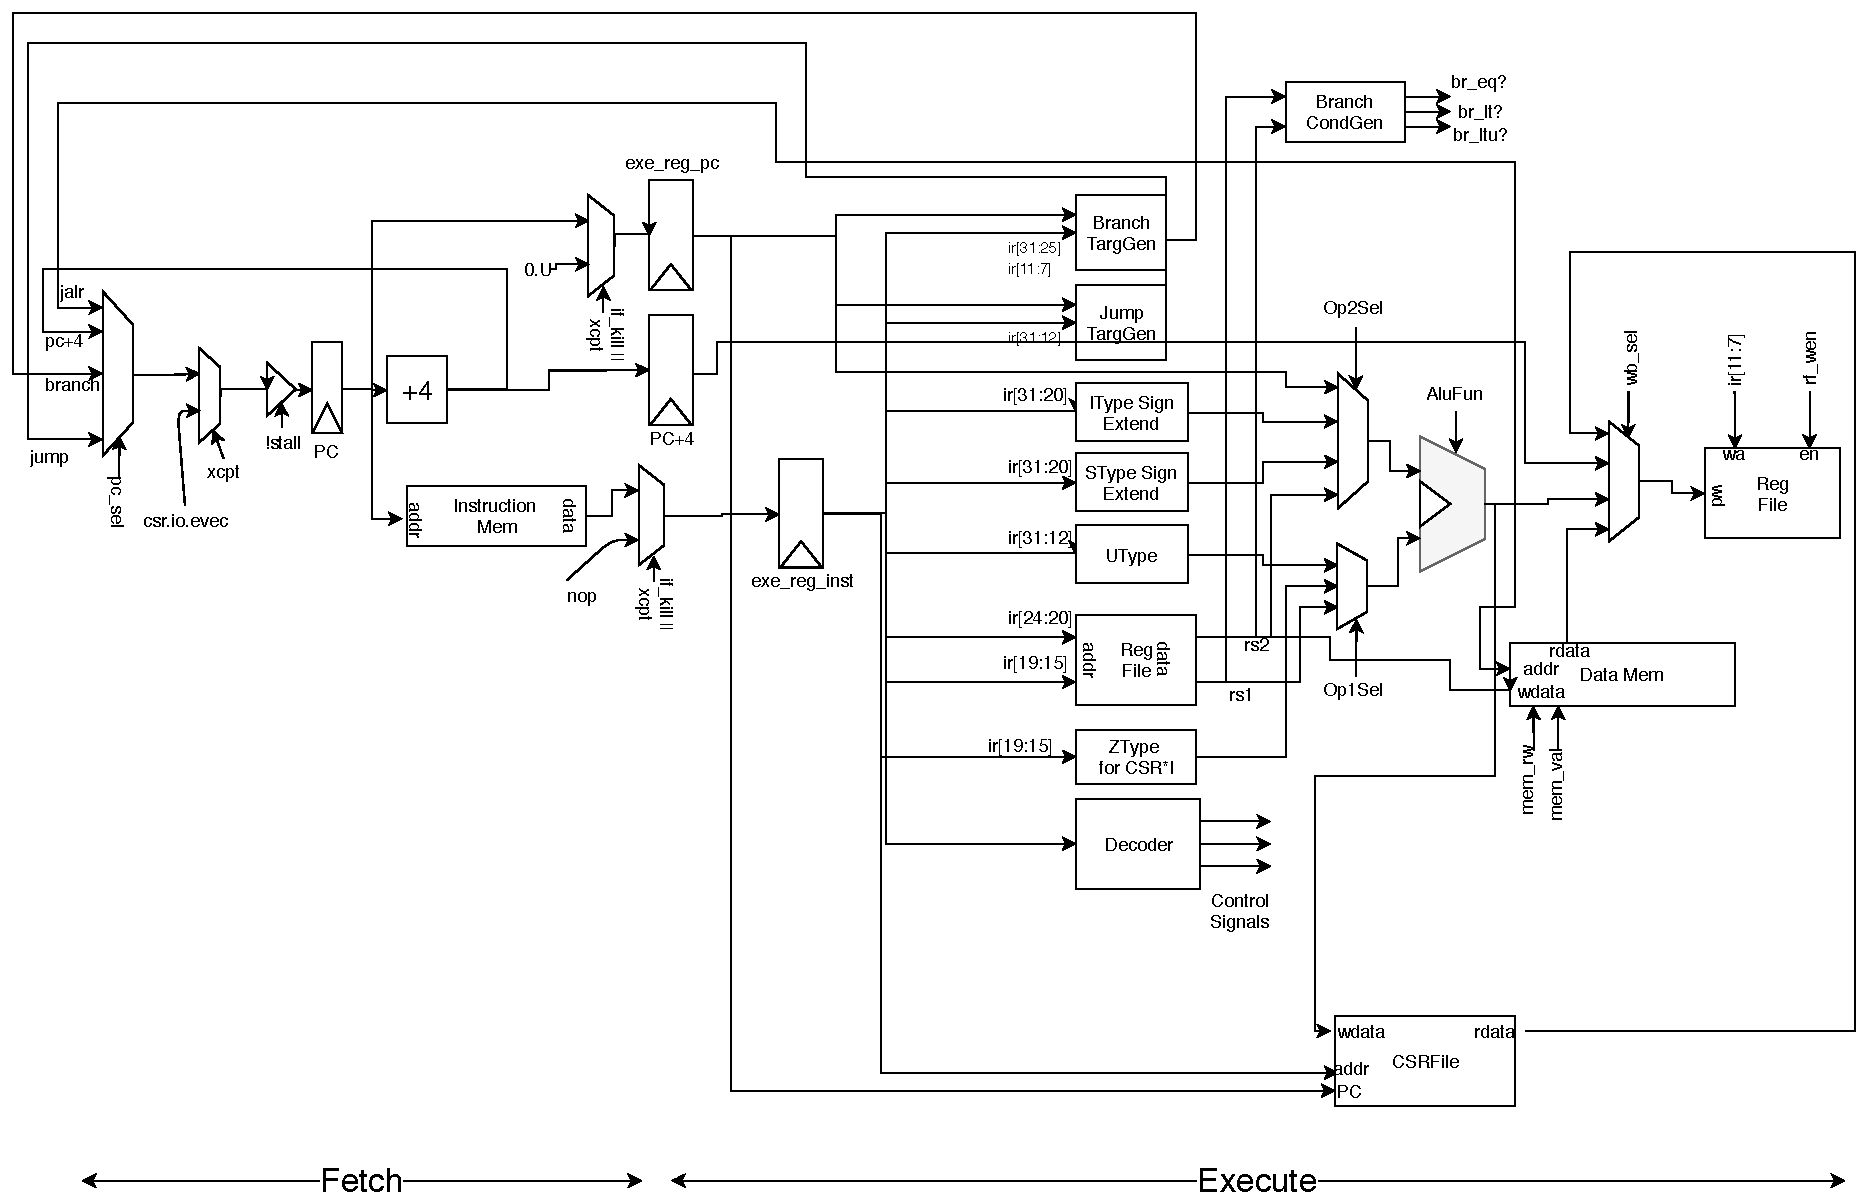
\includegraphics[width=\textwidth]{figures/Introduction/2stage.pdf}
    \caption{Processor structure model -- 2 Stage RISCV core}
    \label{fig:proc_structure}
\end{figure}


\section{Processor-Level Synthesis}

Synthesis of standard processors starts with the instruction set (IS) of the processor.
In order to achieve the highest processor performance this process is done \textbf{manually} since standard processors try to achieve the highest performance and minimal power consumption at minimal cost.
Another reason for synthesizing processors manually is to minimize the design size and therefore fabrication cost for high-volume production, optimize the design as much as possible.
In contrast, the design or synthesis of a custom processor or a custom IP starts with the C code of an algorithm, which is usually converted to the corresponding Control-Data dependency graph, Figure~\ref{fig:c_example}, or FSM model, Figure~\ref{fig:fsm_model}, before synthesis and ends up with a custom processor containing the number and type of components connected as required by the given behavioral model.
This generation is usually called high-level synthesis or occasionally just processor synthesis.
Selecting components and the structure of a PE and \emph{defining register-transfer operations performed in each clock cycle is the task of processor-level synthesis.}

\begin{figure}[h]
    \centering
    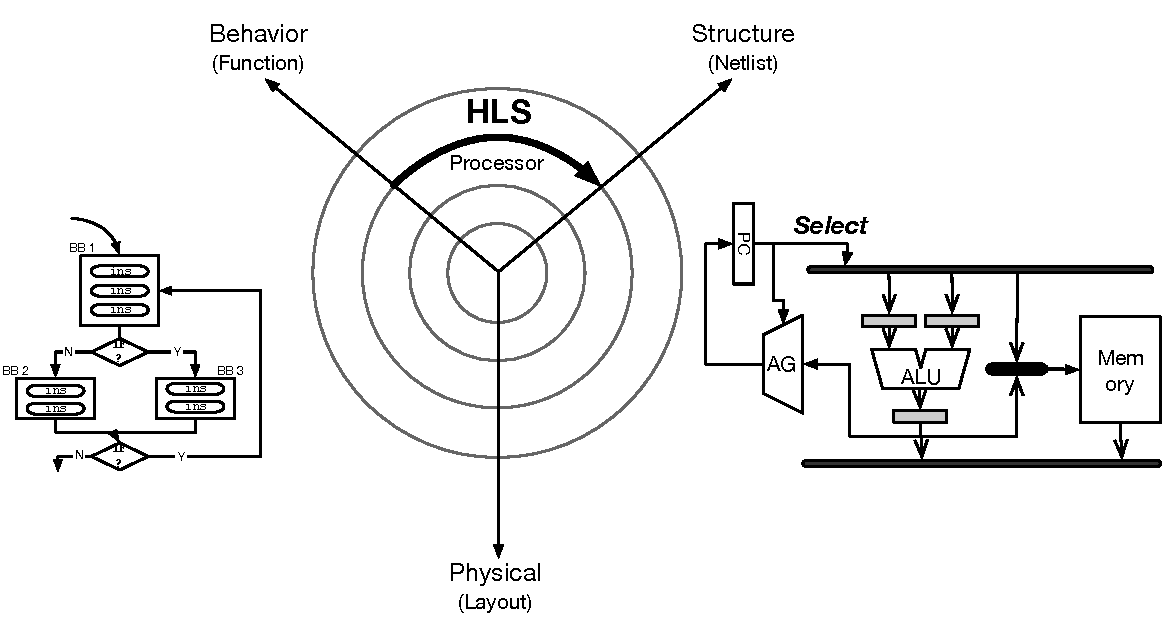
\includegraphics[width=0.9\textwidth]{figures/Introduction/processor-synthesis.pdf}
    \caption{High-Level Synthesis (HLS)}
    \label{fig:proc_synthesis}
\end{figure}

In the process of synthesis there are different tasks that needs to be done to move from behavioral description to structural description.
We briefly enumerate over these tasks, since each of these individual tasks is not the focus of this report.
In this process, the synthesizer needs to decide for component selection base on the input behavior, how these components are connected to each other.
Another important task in the course of synthesis is statically cycle accurate scheduling~\cite{canis_2014_modulo,cong_2009_scheduling,cong_2008_scheduling, cong_2006_efficient}.
Synthesizing control path with either a programmable controller with a read and write program memory or just a read-only memory for fixed-functionality IPs.
And finally, model refinement is the last task that synthesizer needs to do to generate a structural description from a behavioral description.


\section{System-Level Synthesis}

A complete system contains multiple processors and shared resources that they are connected to each other with communication mediums such as buses, network on chips and etc.
To synthesis a system at the behavioral level we need to start with a task graph to express the concurrent behavior of processes.
Figure~\ref{fig:task_graph} shows an example of behavioral description of a whole system model, this description can happen in programming languages that have support for concurrency and synchronization mechanisms.

In Figure~\ref{fig:task_graph} model, there are five processes, P1 to P5.
The system starts with P1, which conditionally triggers either P2 or another process consisting of P3, P4 and P5.
In this subprocess, P3 and P4 runs sequentially and in parallel with P5. In this figure, solid lines indicates sequential dependency, line buffers indicated concurrent relation between processes and dashed lines indicated sync points for parallel processes.
Eventually, when either P2 is finished or the sequential-parallel composition of P3, P4, and P5 is finished, the execution ends.

\begin{figure}[h]
    \centering
    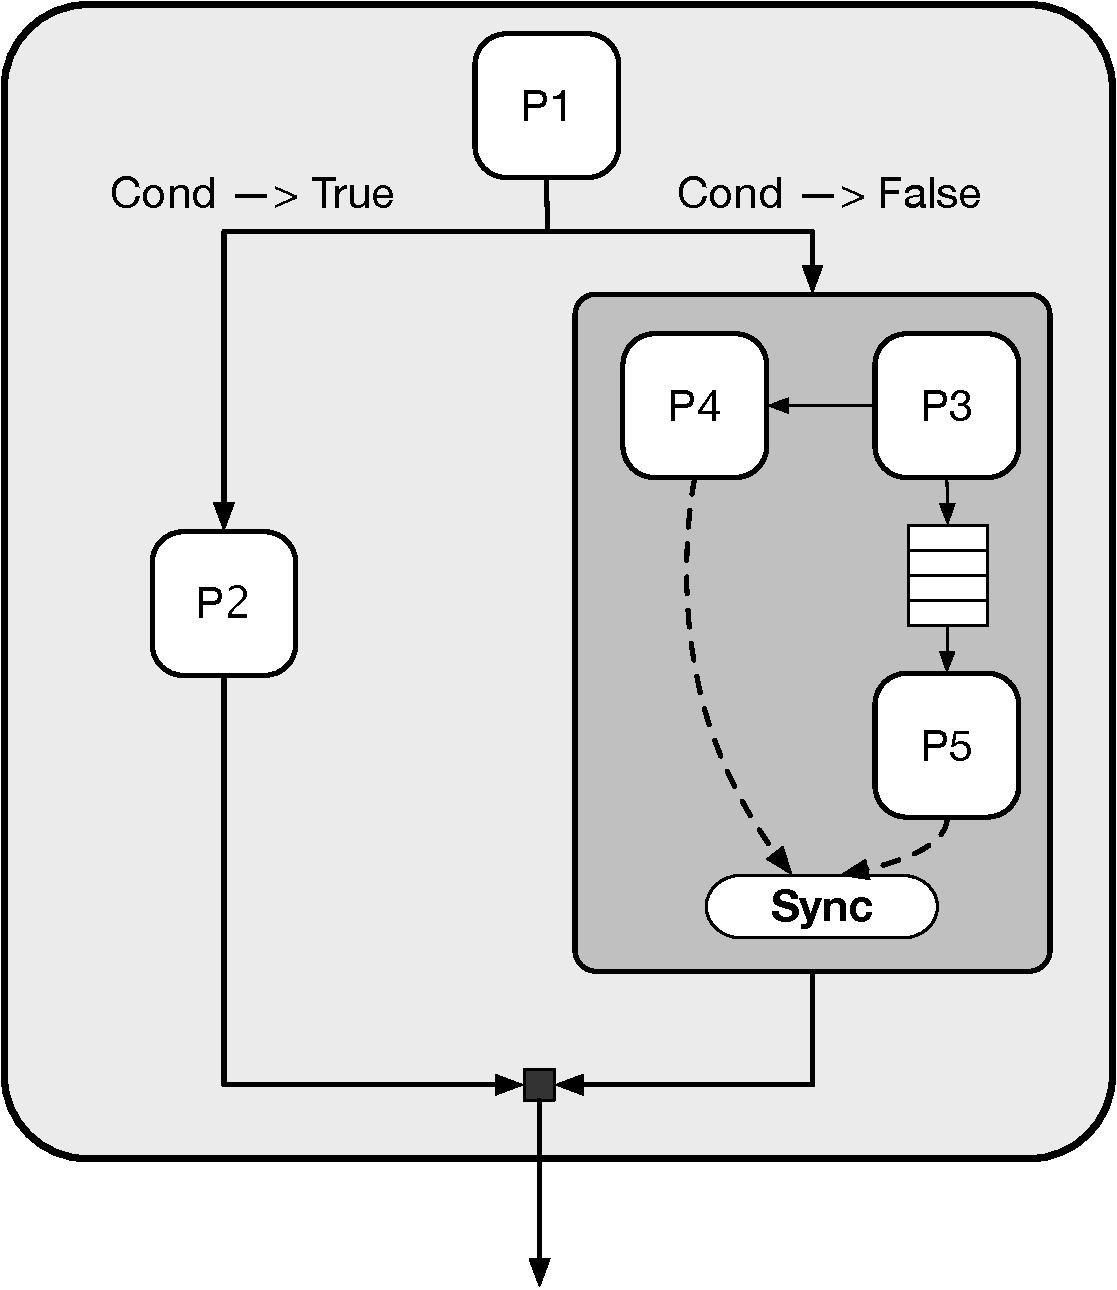
\includegraphics[width=0.55\textwidth]{figures/Introduction/Task_Graph.pdf}
    \caption{System behavioral model}
    \label{fig:task_graph}
\end{figure}


In the synthesis part we need to answer question like what is the memory model. How is the memory shared across different processes.



\subsection{Missing Semantics}
\label{sec:missing_semantics}

A big challenge in \emph{synthesising} is missing semantics. In many cases there are many different representation and design for a same behavioral model. But which model fits better in our design. 
As an example of this problem, we can look in ~\ref{fig:missing_semantics} at a simple case statement available in any hardware or system modeling language.
This type of case statement can be used to model a FSM in which every case such as X1,X2, ..., represents a state in which all its next states are de ned.
This type of case statement can also be used to model a look-up table, in which every case X1, X2, ..., indicates a location in the memory that contains a value in the table.
Therefore,  we can use the same case statement with the same variables and format to describe two completely different components.
Unfortunately, FSMs and look-up tables require completely different implementations:  a FSM can be implemented with a controller or with logic gates, while a look-up table is usually implemented with some kind of memory.
It is also possible to implement a FSM with a memory or a table using logic gates.
However, this would not bea very ef cient implementation, and it would not be acceptable to any designer.
So a model which uses case statements to model FSMs and tables is good for simulation but not for implementation because neither a designer nor a synthesis tool can determine which type of structure was described by the case statement.
The lesson is that contemporary modeling languages allow modelers to de-scribe the design in many different ways and to use the same description for different designs details. But for automatic refinement, synthesis, and veri cation, we need clean and unambiguous semantic which uniquely represents all the system concepts in a given model.  Such a clean semantic is missing from most of the simulation-oriented  languages.
In order to have well defined semantics, we need to introduce some form of formalism to models and modeling languages.


\begin{figure}[h]
    \centering
    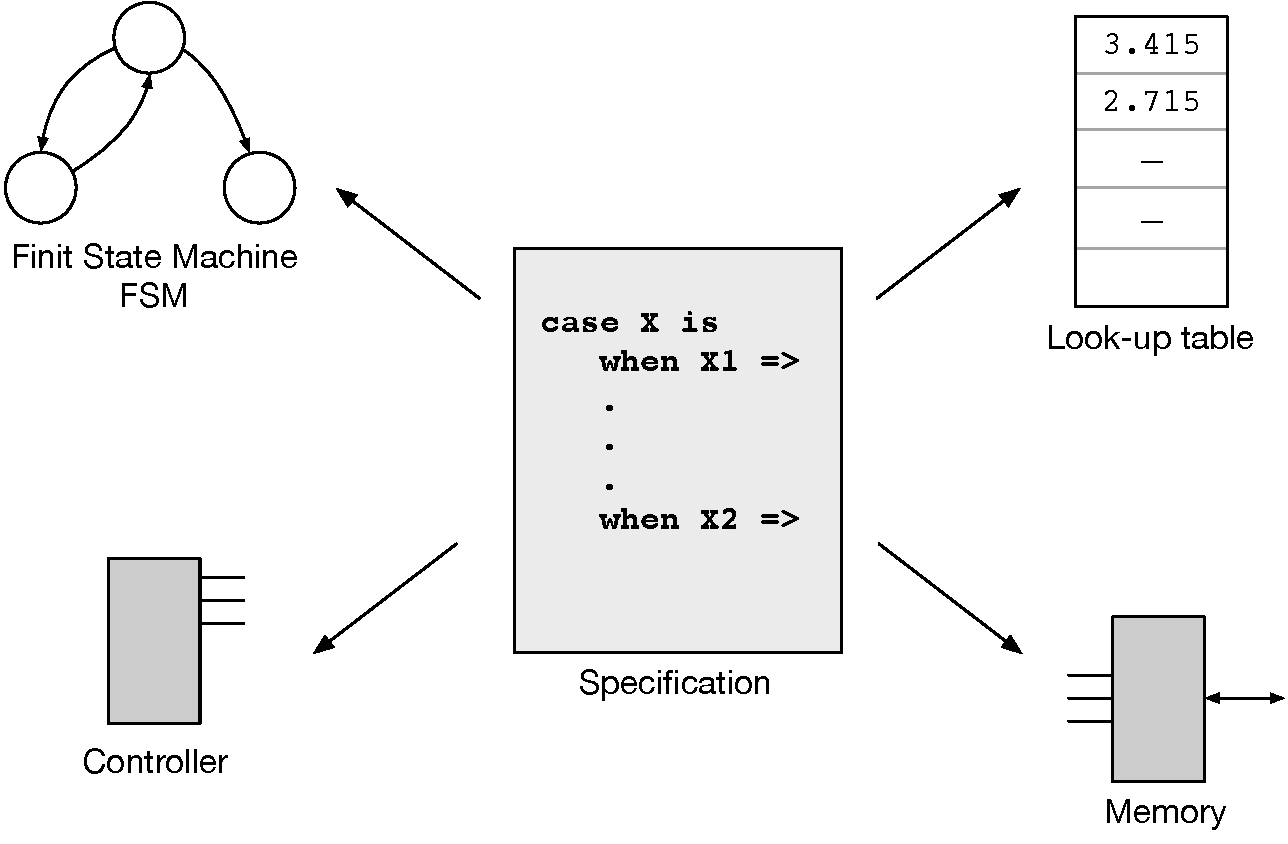
\includegraphics[width=0.7\textwidth]{figures/Introduction/Missing_Semantics.pdf}
    \caption{Missing Semantics}
    \label{fig:missing_semantics}
\end{figure}


\section{Hardware Design Methodologies}

\paragraph{Method1:} Describe-and-Synthesize methodology (late 1980s to late 1990s).
The 1980s brought us tools for logic synthesis which have significantly altered design flow, since the behavior and structure of a design were both captured on the logic level.
Designers specified first what they wanted in Boolean equations or FSM descriptions, and then the synthesis tools generated the implementation in terms of a logic-level netlists.
In this methodology therefore, the behavior or function comes first, and the structure or implementation comes afterwards.
Moreover, both of these descriptions are simulatable, which is an marked improvement over Capture-and-Simulate methodology, because it permits much more efficient verification; it makes it possible to verify the descriptions’ equivalence since both descriptions can in principle be reduced to a canonical form.
However, today’s designs are too large for this kind of equivalence checking.
By the late 1990s, the logic level had been abstracted to the Register-Transfer Level (RTL) with the introduction of cycle-accurate modeling and synthesis.
Therefore, we now have two abstraction levels (RTL and logic levels) and two different models on each level (behavioral and structural).
However, the system gap still persists because there was not relation between RTL and higher system level.

\paragraph{Method2:}  The 1980s brought us tools for logic synthesis which have significantly altered design flow, since the behavior and structure of a design were both captured on the logic level.
Designers specified first what they wanted in Boolean equations or FSM descriptions, and then the synthesis tools generated the implementation in terms of a logic-level netlists.
In this methodology therefore, the behavior or function comes first, and the structure or implementation comes afterwards.
Moreover, both of these descriptions are simulatable, which is an marked improvement over Capture-and-Simulate methodology, because it permits much more efficient verification; it makes it possible to verify the descriptions’ equivalence since both descriptions can in principle be reduced to a canonical form.
However, today’s designs are too large for this kind of equivalence checking.

By the late 1990s, the logic level had been abstracted to the Register-Transfer Level (RTL) with the introduction of cycle-accurate modeling and synthesis.
Therefore, we now have two abstraction levels (RTL and logic levels) and two different models on each level (behavioral and structural).
However, the system gap still persists because there was not relation between RTL and higher system level.


\paragraph{Methode3:}
Specify, Explore-and-Refine methodology (early 2000s to present).
In order to close this gap, we must increase the level of abstraction from the RTL to the system level (SL) and to introduce a methodology that includes both SW and HW.
On the SL, we can start with an executable specification that represents the system behavior; we can then extend the system-level methodology to include several models with different details
that correspond to different design decisions. Each model is used to prove some system property: functionality, application algorithms, connectivity, communication, synchronization, coherence, routing, performance, or some design metric such as performance, power, and so on.
So we must deal with several models in order to verify the impact of design decisions on every metric starting from an executable specification down to the RTL and further to the physical design.
We can consider each model as a specification for the next level model, in which more implementation detail is added after more design decisions are made.
We can label this a Specify-Explore-Refine (SER) methodology [63, 100], in that it consists of a sequence of models in which each model is a refinement of the previous.
Thus SER methodology follows the natural design process in which designers specify the intent first, then explore possibilities, and finally refine the model according to their decisions.
SER flow can therefore be viewed as several iterations of the basic Describe-and-Synthesize methodology.

In order to explain about SER model first we overview the status of methodologies presently in use, their shortcomings, and how to upgrade them to the system level.

